\documentclass[a4paper,11pt]{jsarticle}

%枠設定
\usepackage[margin=25mm]{geometry}
% 数式
\usepackage{amsmath,amsfonts}
\usepackage{bm}
% 画像
\usepackage[dvipdfmx]{graphicx}

\begin{document}

\section*{(1)レーザ変位計によるはりのたわみ測定}

\section{実験目的}
精密情報機器や機械要素等の設計において重要となるはりたわみについて,
レーザ式変位センサを用いて,両端支持ばりのたわみを計測することによって
理解する.

\section{はりたわみの理論}
両端支持ばりのたわみに関する模式図を図1に示す.

\begin{figure}[h]
  \centering
  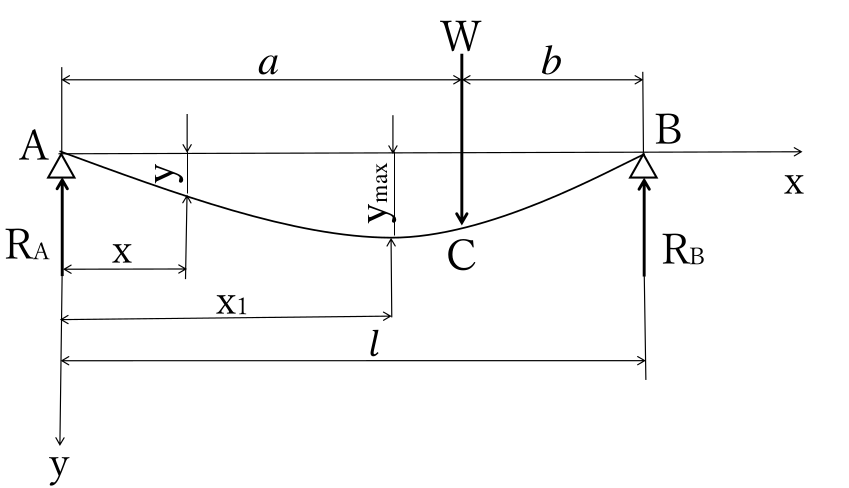
\includegraphics[width=10cm]{AB.png}
  \caption{両端支持ばりの模式図}
\end{figure}
スパン$l$の両端支持ばりABが,左支点Aから$a$,右支点Bから$b$の距離にある点Cに,集中荷重$W$を受ける場合の
最大たわみ$y_{max}$は,
\begin{equation}
  y_{max} = {\dfrac{Wb({l^2}-{b^2})^{3/2}}{9\sqrt{3}EIl}}
\end{equation}
である.ただし,最大たわみを生ずる位置$x_1$は次のようになる.
\begin{equation}
  x_1 = {\sqrt{\dfrac{a(a+2b)}{3}}}={\sqrt{\dfrac{{l^2}-{b^2}}{3}}}
\end{equation}
また,荷重点C$(x=a)$のたわみ$y_c$および中央のたわみ$(y)_{x={1/2}}$は,それぞれ
\begin{equation}
  y_{c} = {\dfrac{Wa^{2}b^{2}}{3EIl}}
\end{equation}
\begin{equation}
  (y)_{x={1/2}} = {\dfrac{Wb(3l^{2}-4b^{2})}{48EIl}}
\end{equation}
である.なお集中荷重$W$がスパンの中央に位置する場合は,
\begin{equation}
  a = b = \dfrac{1}{2}
\end{equation}
であるから,
\begin{equation}
  x_1 = \dfrac{1}{2}
\end{equation}
となり,最大たわみ$y_{max}$が求まる.
\begin{equation}
  y_{max} = {\dfrac{Wl^{3}}{48EIl}}
\end{equation}

\section{実験装置}
\begin{enumerate}
  \item はり構造の力学実験装置(青色のアングルで組まれた装置)\\
  はり\\
  支点\\
  おもり(0.500$kg$:4 個,0.200$kg$:3 個,0.100$kg$:1 個,合計 2.700$kg$)\\
  おもり支持金具(0.224$kg$)
  \item CMOS レーザアプリセンサ\\
  アンプユニット IL-1000\\
  センサヘッド IL-065\\
  電源ユニット KZ-U3
  \item マイクロメータ(最小目盛:0.001$mm$,測定範囲 0-25$mm$)
  \item マイクロメータ(最小目盛:0.001$mm$,測定範囲 25-50$mm$)
\end{enumerate}

\section{実験準備}
\begin{enumerate}
  \item CMOS レーザアプリセンサの電源ユニット KZ-U3 の電源コードをテーブルタップに接続して,
  電源投入後 30 分以上放置する.センサヘッド IL-065[基準距離:65$mm$,測定距離:55-105$mm$]
  からレーザ光(赤色半導体レーザ,可視光,波長 665$nm$)が照射される.なお,レーザ光は直接
  入らないように注意すること.
  \item アンプユニット IL-1000 測定値表示部には,センサヘッドとはり間の距離が小数点以下 3 桁まで
  表示される(単位 $mm$).表示が安定しない場合は,センサヘッドのフィルタガラスが汚れている
  可能性があるため,柔らかい布で拭きとる.
\end{enumerate}

\section{実験方法}
\begin{enumerate}
  \item はりの断面の幅 $b'$,高さ $h$ を左右支点近傍と中央の 3 箇所について,マイクロメータを使って
  小数点以下 3 桁まで測定する.\\
  \quad 断面二次モーメント $I$ は,次式で求められる.
  \begin{equation}
    I = {\dfrac{b'h^3}{12}}
  \end{equation}
  \item スパンの長さ$ l $は,$l= 800[mm] $である.
  \item まずは,左支点 A から集中荷重$ W $の作用点 C までの距離を$a = 500[mm] $とする.
  \item 左支点 A から最大たわみ$y_{max}$を生ずる位置までの距離 $x_1$[$mm$] を式 (2) から求める.
  \item 左支点 A から $x_1$ の位置にセンサヘッド支持台中心を移動させ,はりに対して下側からレーザ光を照射する.
  センサの動作確認 LED ではりとの距離を調整し,測定面に対してセンサの投光面が平行になるように
  設定して固定する.緑 LED が点灯しているときは,はりがセンサの測定範囲に位置しており,測定が可能である.
  \item  集中荷重 $W$ の作用点 $C$ におもり支持金具を取りつける.
  \item アンプユニット IL-1000 の ZERO SHIFT スイッチを押して,表示を ”0.000” にする.\\
  はりにおもり支持金具の重さ(0.224$kg$)の荷重がかかったところが基準になることに,注意すべきである.
  \item はりに荷重を載せていくと,荷重の増加とともにはりとセンサヘッド間の距離が減少する.
  荷重を 0[$kg$] から順に 0.5,1.0,1.5,2.0,2.2,2.4,2.6,2.7[$kg$]と増加させていき,それぞれの
  荷重に対応する最大たわみ$y_{max}$を記録する.
  \item 荷重を 2.7[$kg$]から順に 2.6,2.4,2.2,2.0,1.5,1.0,0.5,0[$kg$]と減少させていき,それぞれの
  荷重に対応する最大たわみ$y_{max}$を記録する.
  \item つぎに,$a= 600[mm],700[mm]$のそれぞれの場合について,4から9までを繰り返す.
\end{enumerate}

\section{実験結果の整理}
・はりのスパン:$l = 800[mm]$\\
\quad・鋼の縦弾性係数(標準値):
\begin{equation} 
  E = 2.06 \times 10^5 [MPa] 
\end{equation}

\begin{enumerate}
  \item はり断面の幅 $b'$ と高さ $h$ を表 1 に記録する.
  \item $a = 500 [mm] $のとき,最大たわみ$y_{max}$ を生ずる位置 $x_1$ は$ 428.2 [mm]$ である.
  荷重を増加させたときの最大たわみ $(y_{max})_i$と,減少させたときの最大たわみ $(y_{max})_d$を,表2
  に記録する.最大たわみの理論値 $y_{max}$は,式 (1) から計算する.また,誤差率$ \delta [\%]$は,
  \begin{equation} 
    \delta = \frac{{\left(\frac{{(y_{\text{max}})_i + (y_{\text{max}})_d}}{2} - y_{\text{max}}\right)}}{{y_{\text{max}}}} \times 100[\%]
  \end{equation}
  から計算する.
  \item $a = 600 [mm] $のとき,最大たわみ$ y_{max}$を生ずる位置 $x_1$は $447.2 [mm] $である.
  2と同様にして,表3に最大たわみ$y_{max}$の値を記録する.
  \item $a = 700 [mm] $のとき,最大たわみ$ y_{max}$を生ずる位置 $x_1$は $458.3 [mm] $である.
  2と同様にして,表4に最大たわみ$y_{max}$の値を記録する.
\end{enumerate}

% ページ1の挿入
\begin{figure}[htbp]
  \centering
  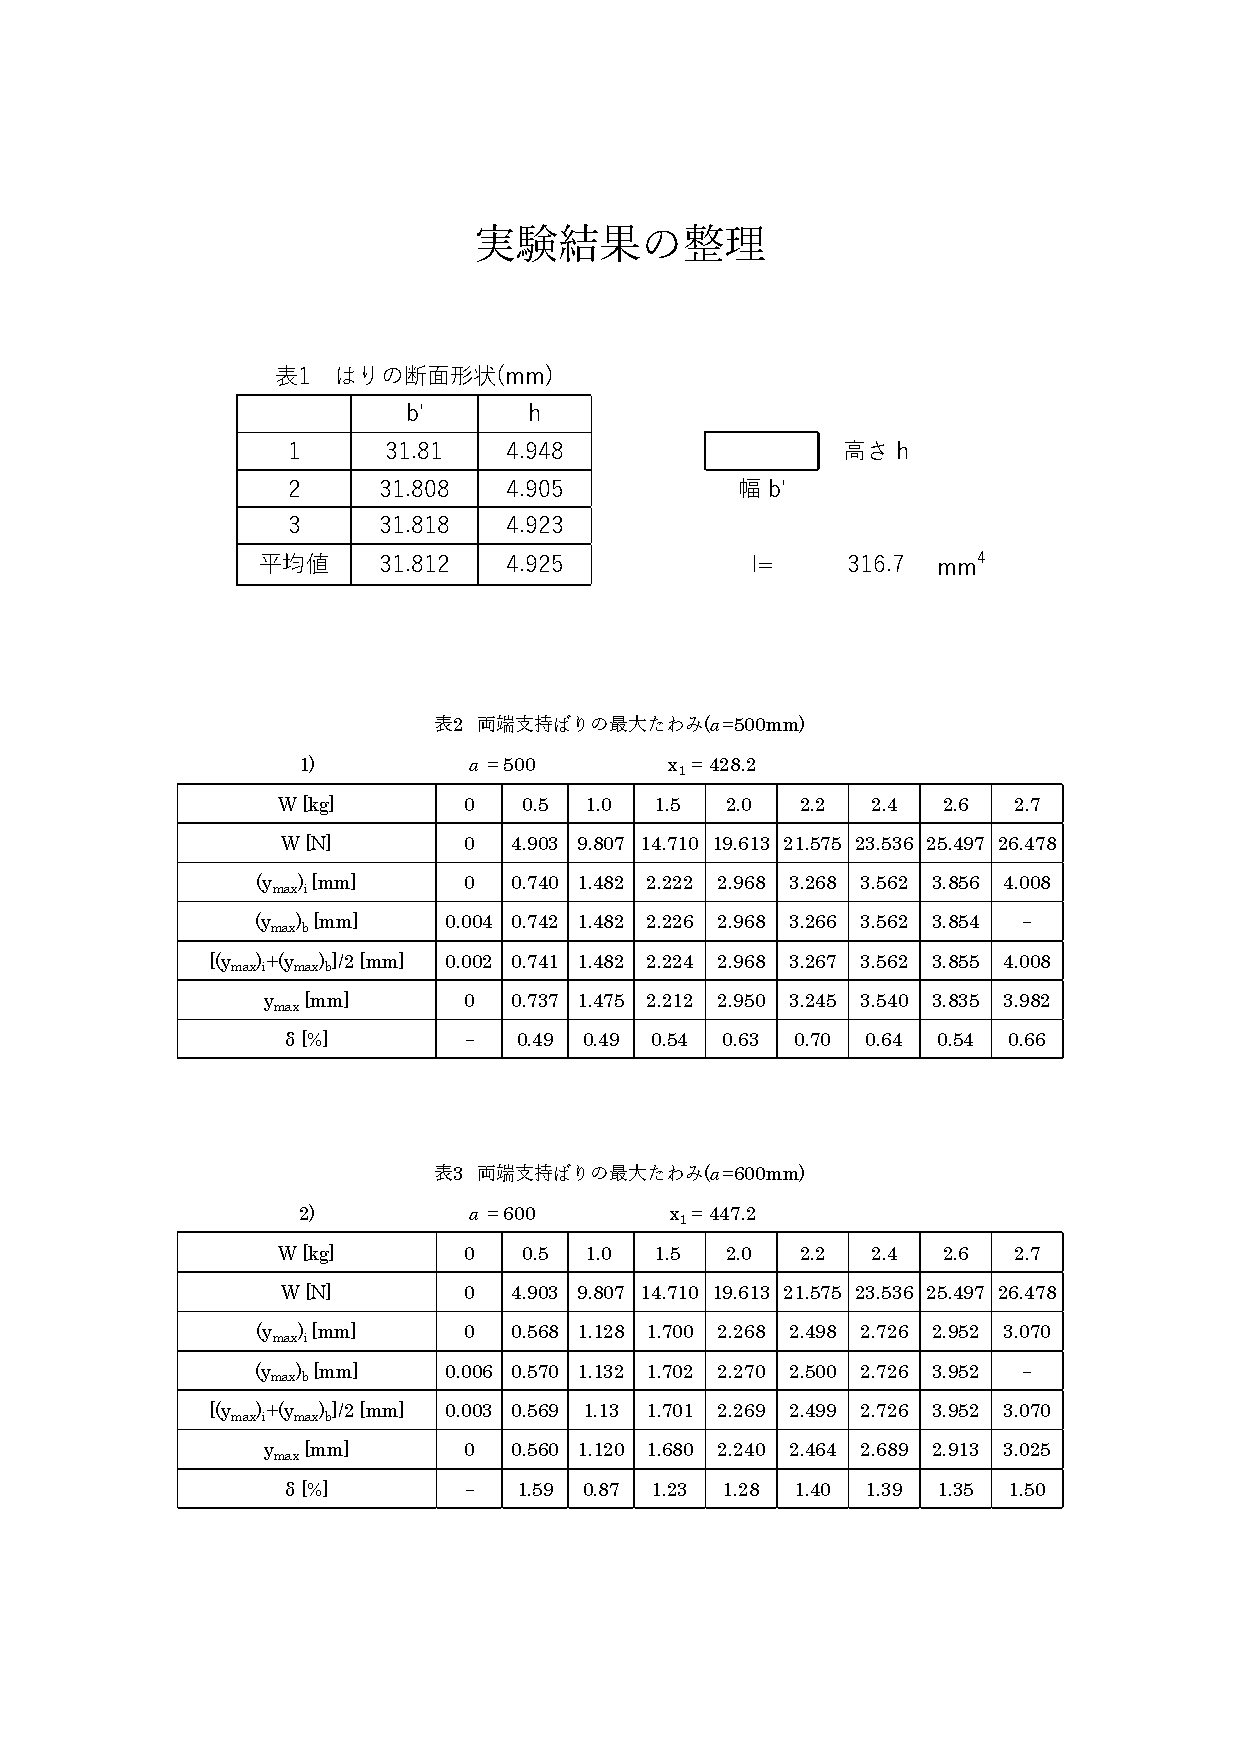
\includegraphics[page=1,width=\textwidth,height=\textheight]{1.pdf}
\end{figure}

\clearpage

% ページ2の挿入
\begin{figure}[htbp]
  \centering
  \includegraphics[page=2,width=\textwidth,height=\textheight]{1.pdf}
\end{figure}
\clearpage


\end{document}